\section{Дифференциальный поиск и прореживание.}

\subsection*{DARTS}

\begin{figure}[H]
	\centering
	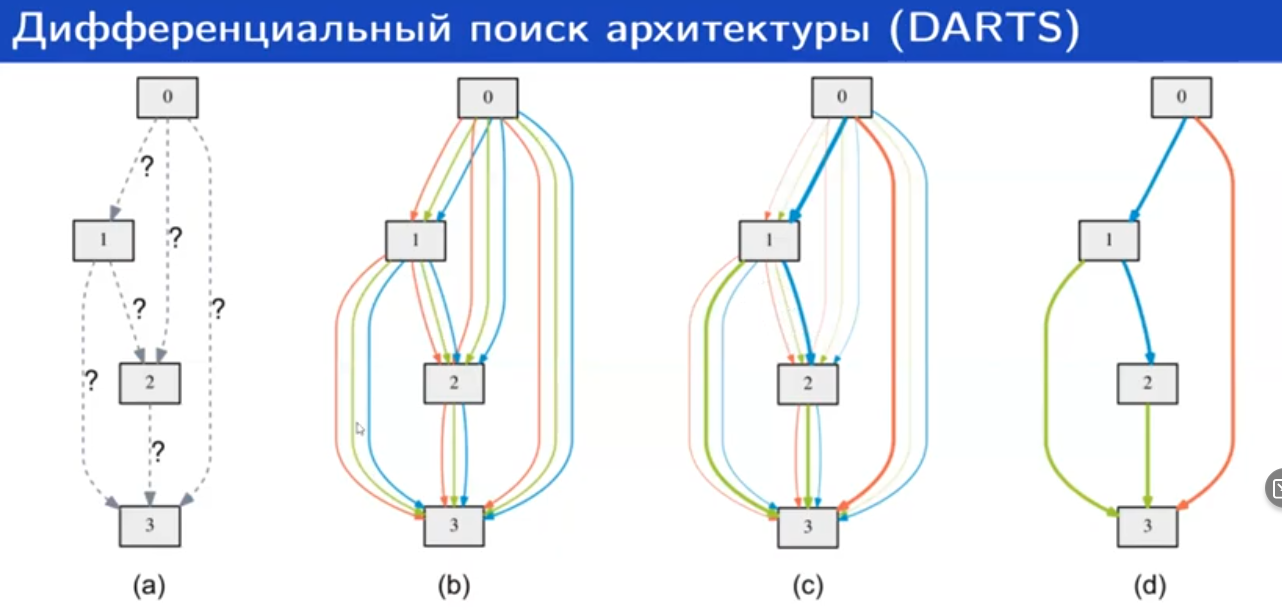
\includegraphics[scale=.4]{images/darts}
	\caption{Дифференциальный поиск архитектуры}
\end{figure}

Есть вершины, ребрами кодируются преобразования. Из каждой вершины
выходят несколько результатов с весами и протаскиваются в следующие
вершины. Затем веса обучаются градиентным спуском и остаются
только значимые пути.

\subsection*{Прореживание}

Относится к residual архитектурам. Можно научиться скипать
содержательные слои, если они не вносят вклад в качество модели.
(возвращают значения около нуля) После удаления преобразований
архитектуру требуется дообучить.

Можно удалять ребра из двудольного графа полносвязной архитектуры.
Полезность ребер определяется по формуле $L_i = \frac{a_i^2}{[H^{-1}]_{ii}}$,
где $a_i$ - значение параметра, $H$ - гессиан. Если дорого
считать гессиан можно брать $|a_i|$.